\chapter{Задание \textnumero1}

\section{Условие}
Реализовать загружаемый модуль ядра, который при загрузке записывает в системный журнал сообщение о запущенных процессах. Модуль должен собираться при помощи Make-файла.

\section{Реализация}
\begin{lstlisting}[caption={Makefile}]
ifneq ($(KERNELRELEASE),)
	obj-m := md.o
else
	CURRENT = $(shell uname -r)
	KDIR = /lib/modules/$(CURRENT)/build
	PWD = $(shell pwd)
default:
	$(MAKE) -C $(KDIR) M=$(PWD) modules

clean:
	@rm -f *.o .*.cmd .*.flags *.mod.c *.order
	@rm -f .*.*.cmd *~ *.*~ TODO.*
	@rm -fR .tmp*
	@rm -rf .tmp_versions

disclean: clean
	@rm *.ko *.symvers
endif
\end{lstlisting}
\begin{lstlisting}[caption={md.c}]
#include <linux/init.h>
#include <linux/sched.h>
#include <linux/module.h>
#include <linux/kernel.h>
#include <linux/init_task.h>

MODULE_LICENSE("GPL");
MODULE_AUTHOR("Faris Nabiev");

static void __exit my_module_exit(void);
static int  __init my_module_init(void);

module_init(my_module_init);
module_exit(my_module_exit);

// Инициализация модуля
static int __init my_module_init(void)
{
   struct task_struct *task = &init_task;

   printk(KERN_INFO "Module task_01: loaded!\n");

   do
   {
     printk(KERN_INFO "Module task_01: "
                      "process: %s - %d, ""parent: %s - %d\n",
            task->comm, task->pid, task->parent->comm, task->parent->pid);
   }
   while ((task = next_task(task)) != &init_task);

   printk(KERN_INFO "Module task_01: "
                    "current: %s - %d, parent: %s - %d\n",
          current->comm, current->pid,
          current->parent->comm, current->parent->pid);

   return 0;
}

// Выгрузка модуля
static void __exit my_module_exit(void)
{
   printk(KERN_INFO "Module task_01: unloaded\n");
}
\end{lstlisting}

\section{Результаты работы}

\begin{figure}[H]
    \centering
    \caption{Сборка и загрузка модуля}
    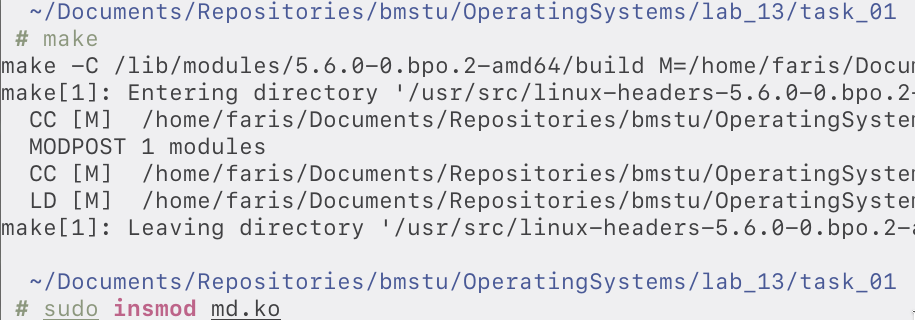
\includegraphics[scale=0.45]{images/src_01.png}
\end{figure}
\begin{figure}[H]
    \centering
    \caption{Проверка списка загруженных модулей}
    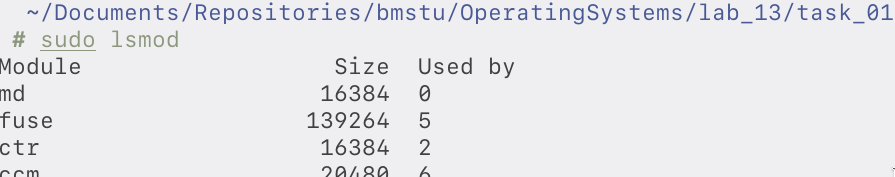
\includegraphics[scale=0.45]{images/src_02.png}
\end{figure}
\begin{figure}[H]
    \centering
    \caption{Вывод буфера сообщений ядра}
    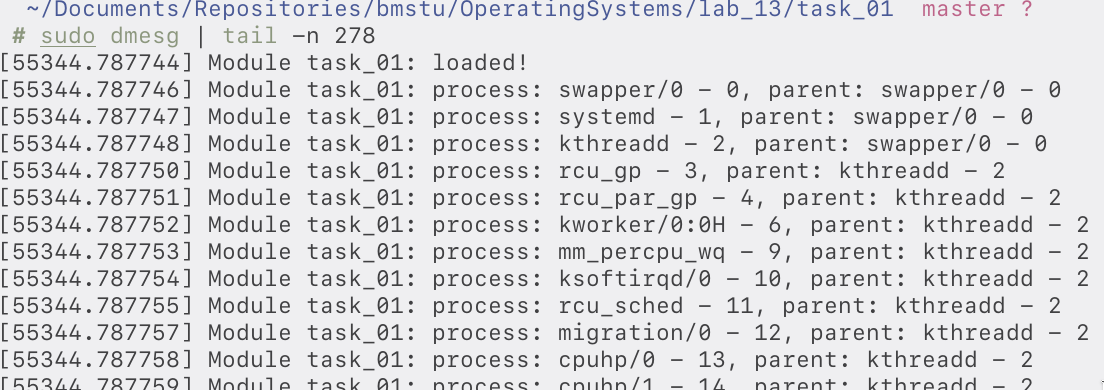
\includegraphics[scale=0.4]{images/src_03.png}
\end{figure}
\begin{figure}[H]
    \centering
    \caption{Выгрузка модуля и проверка буфера сообщений ядра}
    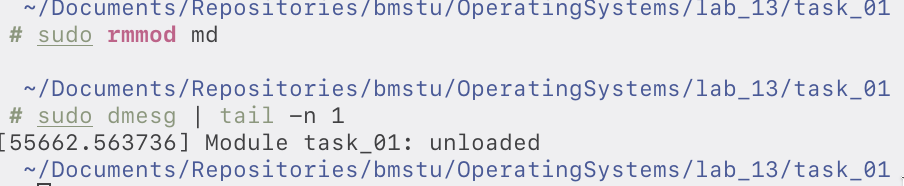
\includegraphics[scale=0.45]{images/src_04.png}
\end{figure}
